%%%%%%%%%%%%%%%%%%%% author.tex %%%%%%%%%%%%%%%%%%%%%%%%%%%%%%%%%%%
%
% sample root file for your "contribution" to a contributed volume
%
% Use this file as a template for your own input.
%
%%%%%%%%%%%%%%%% Springer %%%%%%%%%%%%%%%%%%%%%%%%%%%%%%%%%%


% RECOMMENDED %%%%%%%%%%%%%%%%%%%%%%%%%%%%%%%%%%%%%%%%%%%%%%%%%%%
\documentclass[graybox]{svmult}

% choose options for [] as required from the list
% in the Reference Guide

\usepackage{mathptmx}       % selects Times Roman as basic font
\usepackage{helvet}         % selects Helvetica as sans-serif font
\usepackage{courier}        % selects Courier as typewriter font
\usepackage{type1cm}        % activate if the above 3 fonts are
                            % not available on your system
%
\usepackage{makeidx}         % allows index generation
\usepackage{graphicx}        % standard LaTeX graphics tool
                             % when including figure files
\usepackage{multicol}        % used for the two-column index
\usepackage[bottom]{footmisc}% places footnotes at page bottom

% see the list of further useful packages
% in the Reference Guide

\makeindex             % used for the subject index
                       % please use the style svind.ist with
                       % your makeindex program

%%%%%%%%%%%%%%%%%%%%%%%%%%%%%%%%%%%%%%%%%%%%%%%%%%%%%%%%%%%%%%%%%%%%%%%%%%%%%%%%%%%%%%%%%

\begin{document}

\title*{Generalising Frailty Assumptions in Survival Analysis: a Geometric Approach}
% Use \titlerunning{Short Title} for an abbreviated version of
% your contribution title if the original one is too long
\author{Vahed Maroufy and Paul Marriott}
% Use \authorrunning{Short Title} for an abbreviated version of
% your contribution title if the original one is too long
\institute{Vahed Maroufy  \at Department of Biostatistics, University of Texas Health, Houston, TX, USA \email{vahed.maroufy@uth.tmc.edu}
\and Paul Marriott \at Department of Statistics, University of Waterloo, Waterloo, ON, Canada.  \email{pmarriot@uwaterloo.ca}}
%
% Use the package "url.sty" to avoid
% problems with special characters
% used in your e-mail or web address
%
\maketitle

\abstract*{This paper uses Information Geometry in a practical and important applied
statistical context: Cox regression in survival analysis. We explore the
geometry of the corresponding model space  including its potentially
complex boundary.  The exact manner that frailty terms in Cox's hazard model are specified
has important implications for modelling. For example, it is very common
to assume a gamma frailty for reasons of mathematical tractability and
convenience. In this paper, we examine if there is a cost to having the
gamma as a default option, without further scientific justification. We
take a geometric approach to understanding the effect of precise model
specification. We use a new, highly flexible but statistically
well-behaved, way of specifying the frailty to calibrate modelling
assumptions that are very commonly used in practice. We show that the
gamma frailty assumption has the effect of considerably under-estimating
standard errors when compared to our more general assumptions and,
potentially, introducing bias. We comment on the implications of this. The
survival times of adult acute myeloid leukaemia patients in northwest
England are analyzed.}

\abstract{This paper uses Information Geometry in a practical and important applied
statistical context: Cox regression in survival analysis. We explore the
geometry of the corresponding model space  including its potentially
complex boundary.  The exact manner that frailty terms in Cox's hazard model are specified
has important implications for modelling. For example, it is very common
to assume a gamma frailty for reasons of mathematical tractability and
convenience. In this paper, we examine if there is a cost to having the
gamma as a default option, without further scientific justification. We
take a geometric approach to understanding the effect of precise model
specification. We use a new, highly flexible but statistically
well-behaved, way of specifying the frailty to calibrate modelling
assumptions that are very commonly used in practice. We show that the
gamma frailty assumption has the effect of considerably under-estimating
standard errors when compared to our more general assumptions and,
potentially, introducing bias. We comment on the implications of this. The
survival times of adult acute myeloid leukaemia patients in northwest
England are analyzed}







\section{Introduction}\label{IntroductionCh4}

One of the key insights of Information Geometry  is the  duality which links the exponential and mixture affine structures, \cite{critchley2017information}. Finite dimensional affine structures in the first are exponential families and affine structures in the second determine  identification conditions in mixture models,  \cite{Marriott2002}. This paper takes this fundamental  insight and explores its implications in  a practical and important applied statistical context.    

The motivating example of this paper is a study of the factors which affect the survival times of adult acute myeloid leukaemia patients. This is an example of a problem in lifetime data analysis, \cite{Lawless1981}. One of the most popular tools here is  Cox's proportional hazard model, \cite{Cox1972}. This models the time dependent hazard function, for subject $i$ with covariates $X_i$, as a product
$$
h_i(t) = h_0(t) \exp\{X_i\beta \},
$$ where $h_0(t)$ is the time dependent baseline hazard common to all subjects. This will be treated as a non-parametric nuisance function. The second term is a time independent  function of the explanatory variables, which is modelled parametrically. Under the proportional hazard  assumption the interest parameters can be estimate using a partial likelihood. Often though there are unmeasured individual level covariates which need to be taken into account in the analysis. This is commonly done by adding  subject level  terms $\theta_i$ in the adapted hazard given by (\ref{Exp_hazard}). Since this will give a parameter for each subject it is convenient to treat these as unobserved  random effects, or {\em  frailties}, and simply estimate parameters associated with the distribution of these terms. 

This  means that we work by mixing over different hazard functions and the key  model choice issue is the specification of the frailty distribution.  It is  here that Information Geometry plays a role through consideration of the fundamental mixture geometry  and its impact on  inference of the parameters of interest. In particular we use  tools associated with  the {\em local mixture model}, see  \cite{Marriott2002}, \cite{anaya2007local}. Of special geometric interest  is the potentially complex boundary that these models can have. For example   \cite{Maroufy2015} shows that local mixture models can have a boundaries which are boundaries of  polytopes or  can be  a non-smooth union of a finite number of smooth components.




Frailty models have been studied by many researchers;
for example,  \cite{Clayton1978},  \cite{Hougaard1986a}, \cite{Klein1992}, and \cite{Gorfine2006}. 
Various hazard models, including Cox's regression model, have
been generalised by assuming a  random  frailty variable.  The frailty model is commonly chosen to return a tractable marginal likelihood
function; hence, gamma, inverse
Gaussian and positive stable distributions  with closed-form Laplace transformations
are regular choices (\cite[p.77]{Cook2007}). Among these the gamma is the most popular model choice,  
(\cite{Klein1992}; \cite{Nielsen1992}; \cite{Vaupel1979}). 

 The goal of this paper is to investigate what might be the  cost  of
specifying a particular parametric form, specifically the gamma, for the frailty distribution when  this choice has been made purely for convenience.  Model uncertainty is a critical problem in applied statistics, and -- as we do here --  the analysis can be treated in a geometric way. The use of geometry in the area is not new, for example the  paper \cite{copas2005local} provides an intriguing solution by proposing  the `double the variance' method for addressing the possibility of undetectably small departures from the model.  Much more detail on the geometry of model specification  can be found in \cite{Anaya2016CIG}.


We investigate the choice of a gamma frailty by calibrating it to a much more general space of mixtures, which can be used as a bench-marking  tool. We use the excellent study of
\cite{Henderson2002} to illustrate these effects in a real context. We  show that 
making  the gamma frailty assumption can have the effect of considerably under-estimating standard errors and its potential
misspecification gives rise to  important biases.  



In general with mixture models, and specifically with the frailty models considered here, the analyst has to balance flexibility with   inferential and computational tractability. In this paper we  use the recently defined {\em discrete mixture of local mixture models}, introduced in \cite{Maroufy2016a}, to achieve the  calibration.  This new model
 generates  a finite dimensional and suitably  parameterized space as a high quality approximation  to a general mixture model with unknown mixing
mechanism. The model is  always identifiable and estimable, and its geometric and inferential properties allow for
fast and efficient estimation algorithms.  These properties make it suitable as a calibration tool, and we are currently exploring using it as a frailty model in its own right.





Notation, motivation and the main results of the paper, including our proposed method
are presented in Section \ref{Methodology}.  Section \ref{Application to frailty modelling} looks at the calibration, with  \S  \ref{Simulation} showing a
simulation study, illustrating that the local mixture method returns similar biases, but larger --
often more than double -- standard deviations for the estimates compared to the Expected-Maximization method
of \cite{Klein1992} where a gamma frailty is assumed. This shows the  considerable impact that fixing on a particular parametric form has on inference, and clearly illustrates that the reduction in standard error may be just an artefact of modelling choice rather than real.
 In Section \ref{Example_survival}, the survival time of 1043
adults acute myeloid leukemia patients, recorded between 1982 and 1998 in northwest England, is analyzed, again with important differences in  inferential conclusions being found.
The paper  closes with a short discussion in Section \ref{Summary}.

\section{Methodology}\label{Methodology}
Throughout this section, we follow the notation and definitions in \cite{Lawless1981} and \cite{Gorfine2006}.
Let $(T^0_{i},C_{i})$, for $i=1,\cdots,n$, be the failure time and censoring time of the $i$th individual,
and also let $X$ be the $n\times p$ design matrix of the covariate vectors. Define $T_i = \min(T^0_{i},C_i)$
and $\delta_i=I(T^0_{i} < C_i)$, where $I(\cdot)$ is an indicator function. In addition, associated with the $i$th
individual, an unobservable covariate $\theta_i$, the frailty, is assumed, where $\theta_i$'s follow some
distribution, $Q$.
Adapting the proportional hazard model of \cite{Cox1972} for the $i$th individual, conditional on the frailty $\theta_i$,
the hazard function is, 
\begin{eqnarray}
h_i(t)=\theta_i\, h_0(t) \exp\{X_i\beta \},\label{Exp_hazard}
\end{eqnarray}
where $h_0(t)$ is the base hazard function, $X_i$ is the $i$th row of $X$ and $\beta=(\beta_0,\cdots,\beta_{p-1})^T$
is a $p$-vector regression coefficients. The cumulative hazard  and survival functions are, respectively, defined as
$
H_i(t)=\int_{0}^{t}{h_i(u)\,du},$ and  $S_i(t)=\exp\{-H_i(t)\}$,
with the base cumulative hazard function $H_0(t)$. We also assume that the frailty $\theta$ is independent
of $X$, and further that, given $X$ and $\theta$, censoring is independent and noninformative for $\theta$
and $(h_0,\beta)$, see \cite{Gorfine2006}. The full likelihood function for the parameter vector $(\beta, H_0)$ is written as
\begin{eqnarray}
 L(\beta,H_0,Q)={\prod_{i=1}^{n}  \int \left[\left(\theta\, h_0(T_i)\, e^{X_i \beta}\right)^{\delta_i} \exp \left\{-\theta\,H_0(T_i)\, e^{X_i \beta}\right\}\right] dQ(\theta)  }.\label{likelihood_frailty} 
\end{eqnarray}


In a similar way to a general mixture model problem,  frailty survival
models with an unknown frailty distribution, suffer from identification and estimability  issues. Although, when all the covariates
variables are continuous with a continuous distribution, \cite{Eleber1982}, show that, given the distribution
of the time duration variable, all the three multiplicative factors are, at least formally, identified. This theoretical result does
not solve the identifiability issue in the general sense. For instance, when there is a discrete covariate
then identifiability requires the corresponding regression coefficient to be limited to a known compact set
\cite[Ch.2]{Horowitz2010}. 

\subsection{Local and global mixture models}\label{Local Mixture Method}


To allow full generality of the mixture structure it  is tempting to only restrict $Q$ to be a finite discrete distribution with an unknown number of components., i.e. 
$$
Q(\theta) = \sum_{i=1}^N \rho_i \delta_{\theta_i}(\theta),
$$ where $\delta$ is the indicator function, and $\sum_{i=1}^N \rho_i =1$ and $ \rho_i > 0$.
Indeed, as shown
by \cite{Lindsay1995}, the non-parametric maximum likelihood estimate of $Q$ lies in such a family. In that case the perturbation space would be `parameterised' by $N$, the number of components, $(\theta_1, \dots, \theta_N)$, the components, and  $(\rho_1, \dots, \rho_N)$, the mixing weights. However, this parameterization  has many problems in implementation. Specifically,  it is poorly identified and has complex boundaries.  A key problem is that mixture components may be too  close to one another to be  resolved with a given set of data and so the order of the finite mixture is essentially not estimable, see \cite{Maroufy2016a}. 


The case where there is a  single  set of  closely grouped components -- or the  much more general situation where $Q$ is
any small-variance  distribution  -- is exactly the case which motivated  the design of the local mixture model (LMM),  see \cite{Marriott2002},
and \cite{Anaya-Izquierdo2007}. The key idea is, essentially,  to  replace the unknown number of clustered mixing components with a fixed number of low order moments parameterised in an inferentially  `nice' way.   The geometric  intuition is that for  a local perturbation all the mixing component distributions will lie close to a low dimensional linear (affine)  space. This space is  spanned by derivatives of the prior and parameterised with a small number of identified parameters.
\begin{definition}\label{Definition 1}
For a density function,  $f(y;\theta)$, belonging to the exponential family, the local mixture model of order $k$, centred at $\vartheta$, is defined as
\begin{eqnarray}
g_{\vartheta}(y;\lambda)=f(y;\vartheta)+\sum\nolimits_{j=1}^k \lambda_j f^{(j)}(y;\vartheta),\hspace{1cm}
\label{one_LMM}
\end{eqnarray}
where $\lambda := (\lambda_1,\cdots,\lambda_k) \in \Lambda_{\vartheta}$, $f^{(j)}(y;\vartheta)=\frac{\partial^j f(y;\theta)}{\partial \theta^j}
\mid_{\theta=\vartheta} $. The parameter space, $\Lambda_{\vartheta}$, is defined by
$$
\Lambda_{\vartheta} := \left\{ \lambda \,|\, g_{\vartheta}(y;\lambda) \ge 0, \,\forall y \right\}
$$
is  convex   with a  boundary determined by the non-negativity of (\ref{one_LMM}). The structure of this boundary is the union of smooth manifolds and is studied in \cite{Maroufy2015}.
\end{definition}
 In \cite{Maroufy2016a}, local mixtures  are 
generalised to  discrete mixtures of
local mixture models.   In Definition \ref{Definition 1} the point $\vartheta$ is fixed, selected by the analyst. This has the natural generalisation to have a set of possible centres,   $\vartheta_1,\cdots\vartheta_L$,   selected independently of the data. This gives rise to the following.
\begin{definition}\label{Definition 2}
The discrete mixture of local mixture
models is defined by
\begin{eqnarray}
g(y;\underline{\vartheta},\underline{\lambda})=\sum\nolimits_{l=1}^L \rho_l\, g_{\vartheta_l}(y;\lambda^l), \label{DMLMM}
\end{eqnarray}
where  $\underline{\lambda}=(\lambda^1,\cdots,\lambda^L)$, $\underline{\vartheta} =( \vartheta_1, \dots, \vartheta_L)$, $\rho_l\geq 0$ and $\sum_{l=1}^{L}\rho_l=1$.
 \end{definition}
 The model selection task with such models is to select $k, L$ and $\vartheta_1,\cdots\vartheta_L$ to balance estimability with the quality
 of approximation to a completely general mixture.  We use the results of \cite[Section 2.1]{Maroufy2016a} which show, for a given value of $k$, how to select the points $\vartheta_1 < \dots < \vartheta_L$  to have a uniform  $L^1$-bound on   the difference between $g(y;\underline{\vartheta},\underline{\lambda})$ and any mixture with mixing distribution $Q$ whose support lies in a compact region containing  $\{\vartheta_1, \dots,  \vartheta_L\}$.
 
 We emphasis,  before we show some of the details in an example, that in this paper, we are using the LMM structure as a calibration tool, in order to evaluate the effect of selecting a particular parametric frailty model. We are generating a rich , but well behaved, class of mixtures which subsume the gamma assumption. 

\begin{example} To illustrate the flexibility of this framework, Figure \ref{newfigsfig1.pdf} shows some discrete mixtures of local mixture
models for the exponential distribution on both the density and hazard scales. Using the methods of \cite[Section 2.1]{Maroufy2016a}  some straightforward numerical analysis shows that selecting points, in the rate parametrisation, at 
$\vartheta_1=0.5,  \vartheta_2=1,\vartheta_3=2$ and $\vartheta_4=3.5$ and fixing $k=4$ gives  excellent $L^1$-approximations for all mixtures $Q$ with support in $[0.3, 5]$. In the figure Model 1 is the unmixed exponential model, Model 2 is a single component local mixture centered at $\vartheta_2=1$, Models 3 and 4 are two components mixtures of local mixture centred at $(1,3.5)$  and  $(0.5,1)$, respectively. 



\begin{figure}[b]
\sidecaption
% Use the relevant command for your figure-insertion program
% to insert the figure file.
% For example, with the graphicx style use
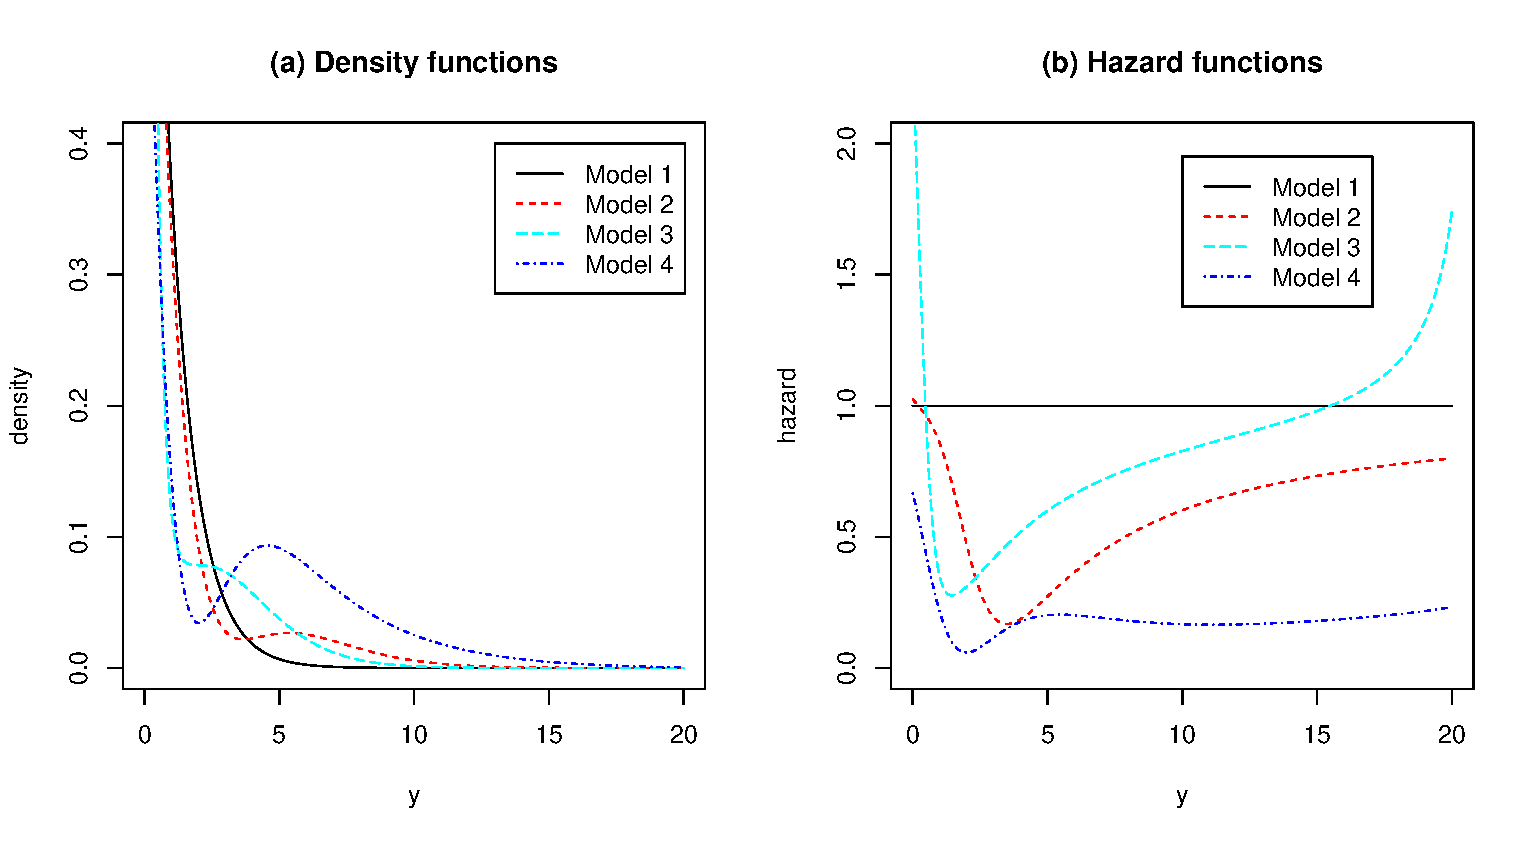
\includegraphics[scale=.45]{newfigsfig1}
%
% If no graphics program available, insert a blank space i.e. use
%\picplace{5cm}{2cm} % Give the correct figure height and width in cm
%
\caption{The flexibility of the model class: (a) four models on a density scale, (b) the same models' hazard functions.}
\label{newfigsfig1.pdf}       % Give a unique label
\end{figure}

\end{example}
In  \cite{Maroufy2016a}  it was shown that an adaptation of the EM algorithm works well for fitting a finite mixture of local mixtures. We   only consider here local mixture models
of order $k = 4$. Increasing this degree -- while mathematically possible -- only adds a small marginal improvement to the local
modelling performance, (\cite{Marriott2006}), at the cost of extra parameters. 

The key, novel, issue in the estimation is to deal with the fact that the parameter space, $\Lambda_{\vartheta}$, has a complex boundary. For this paper, for the Cox model,  we need to  consider the case where $f(y;\theta) =\theta\exp(-\theta y)$ and then the  parameter space is characterized as the set of all 
$\lambda$'s such that, for all $y>0$,
\begin{equation}\label{supp_poly}
\vartheta \lambda_4 y^4-(4 \lambda_4+\vartheta \lambda_3) y^3+(3\lambda_3 + \vartheta \lambda_2)y^2-(2 \lambda_2+\vartheta \lambda_1) y+ \lambda_1+\vartheta \ge 0.
\end{equation}
The boundary is characterised as being the cases where  (\ref{supp_poly}) has  only repeated positive roots, and it can be shown, by direct calculation, that the parameter space is the union of smooth manifolds.   This characterisation allows explicit parameterisations of the component manifolds to be computed and these are exploited in the numerical studies of this paper. See Appendix for details. 

\section{Application to frailty modelling}\label{Application to frailty modelling}

In this section, we investigate the size of the effect on inference associated with fixing on a particular frailty
distribution by comparing a standard gamma frailty model to our more general local mixture approach.  In cases where
the only reason for selecting a gamma frailty was convenience  we argue differences, such as a reduction in standard
error, are artefacts of  model choice and not real.  In order to investigate the best possible case for the gamma
frailty assumption we simulate, in \S \ref{Simulation}, from that frailty distribution, and we only make the comparison
to  a one component  local mixture with $k=4$. Even with these restrictions we see that standard errors associated with
the gamma assumption are considerably smaller than those of the LMM.   Furthermore, in  the real data example of \S \ref{Example_survival},
it turns out that the $k=4$, one component  local mixture is the appropriate choice for that data and   we find important
inferential differences which might be due to either  misspecification   bias,  or artificially reduced standard errors,
in the gamma based model. 



Intuitively, for any fixed $\vartheta$, the finite dimensional parameter vector $\lambda$ represents
the frailty distribution through its central moments. Local mixing also can be seen as a mechanism that
extends a parametric model to a larger and more flexible space of densities which has nice geometric
and inferential properties,  allowing calibration of a particular parametric assumption.
\noindent
Substituting the local mixture expansion  of Equation (\ref{one_LMM}) we obtain
\begin{eqnarray}
l(\beta,H_0, \lambda)&=&\sum\nolimits_{i=1}^{n}{\left(\delta_i[\log h_0(T_i)+ X_i \beta]+ \log f(T_i,\beta,\vartheta)\right)}\nonumber\\ 
 &&+  \sum\nolimits_{i=1}^{n}\log \left( 1+\sum\nolimits_{j=1}^{k}{\lambda_j\, A_{j}(\delta_i,y_i)} \right), \hspace{1cm} \lambda\in \Lambda_{\vartheta}\label{log_like_exp1}
\end{eqnarray}
in which $A_{j}(\delta_i,y_i)= \frac{f^{(j)}(T_i,\beta,\vartheta)}{f(T_i,\beta,\vartheta)}$,
and $y_i=H_0(T_i) e^{X_i \beta}$. We maximize Equation (\ref{log_like_exp1}) when 
estimating $\beta$, where $H_0$ and $\lambda$ are considered as nuisance parameters. Thus, a profile likelihood optimization method is
employed. That is, we first maximize for $\lambda$ over $\Lambda_{\vartheta}$ to obtain $\hat{\lambda}$ 
and impute $\hat{H}_0$ for $H_0$, then maximize $l_p(\beta)=l(\beta,\hat{H}_0,\hat{\lambda})$ to estimate $\beta$.

To impute $h_0(t)$ and $H_0(t)$ we  use the arguments in \cite{Gorfine2006}
to provide a recursive estimate of the cumulative hazard function using the fact that for two consecutive failure times,
$T_{(i)}$ and  $T_{(i+1)}$, we have $H_0(T_{(i+1)})=H_0(T_{(i)})+\Delta H_i$. Substituting this recursive
equation into the log-likelihood function in (\ref{log_like_exp1}), considering the conventions in \cite{Breslow1972} and
taking partial derivative with respect to $\Delta H_i$, we obtain 
\begin{eqnarray}
\frac{\partial l}{\partial \Delta H_i}=\frac{1}{\Delta H_i}-\sum_{\ell=i}^{n}e^{X_\ell \beta}+\frac{P^{\prime}(e^{X_i\beta}[H_0(T_{(i)})+\Delta H_i])}
{P(e^{X_i\beta}[H_0(T_{(i)})+\Delta H_i])},\label{partial_diff} 
\end{eqnarray}
which is a function of just $\Delta H_i$ when $\hat{H}_0(T_{(i)})$ is given at time $T_{(i+1)}$, $P(\cdot)$
is a polynomial of degree four with its coefficients  linear functions of $(\lambda_1,\lambda_2,\lambda_3,\lambda_4)$ and $P^{\prime}(\cdot)$
is its derivative with respect to $\Delta H_i$.
When the denominator is not zero, Equation (\ref{partial_diff}) is a polynomial of degree five which can be solved numerically
for $\Delta H_i$. Note that when there is no frailty factor --  that is $\lambda=(0,0,0,0)$ --  then the last term in equation
(\ref{partial_diff}) is zero, and the estimate of the cumulative hazard function reduces to the form in \cite{Johansen1983}
which is the estimate in \cite{Klein1992} with $\hat{\omega}=1$.


\subsection{Simulation Study}\label{Simulation}
In this section, a simulation study  illustrates  the  effect of making  the    gamma frailty assumption  when compared to the much richer  local mixture
method. We adapt the method in \cite{Klein1992}, which assumes a gamma model with mean
1 and variance $\eta$ for the frailty, and apply the Expectation-Maximization algorithm.

We let $C=0.01$, $\tau=4.6$ and we follow a similar set-up as found in \cite{Hsu2004}. For each individual
the event time is $T=[ -\log(1-U) \{  \theta \exp\{\beta X\} \}^{-1}] ^{-1/\tau} C^{-1}$, where
$X\sim N(0,1)$, $U\sim$ uniform$[0,1]$. The censoring distribution is $N(100,15)$, and frailty
is assumed to follow a gamma distribution with mean 1 and variance $\eta$. Table \ref{simulLMMnew}
shows the bias and standard error for the estimates of the regression coefficient using both
methods for three different values of $\eta$. It is clear that the local mixture method, which
does not use any information about the frailty model, returns very similar biases as the Expectation-Maximization method for the gamma frailty. However, the standard deviation for the estimates in the local mixture method are almost twice as large as these
for the Expectation-Maximization method.  

\begin{table}[h!]
\caption{Bias and standard errors of coefficient estimates, when frailty 
is generated from $\Gamma(\frac{1}{\eta},\eta)$. LMM is the local mixture method; Gamma the 
Expectation-Maximization method for the gamma frailty.}
\label{simulLMMnew}
\begin{center}
\begin{tabular}{c c c c c c c}

\hline %\hline 
& & &\multicolumn{2}{c}{Gamma } & \multicolumn{2}{c}{LMM}\\ [0.3ex]
\hline
$n$ & $\eta$ & $\beta$ &  $bias$ & $std$ & $bias$ & $std$ \\ [0.3ex]% & iterate 
\hline 
%200 & 0.1&  $\log{3}$ & -0.018  & 0.134 & 0.022 & 0.149 \\ %& Yes\\
200 & 0.5&  $\log{3}$ & -0.057  & 0.18 & -0.048 & 0.43 \\ %& No\\
%200 & 0.2&  $\log{3}$ & -0.030  & 0.125 & 0.028 & 0.148 \\ % & Yes\\
200 & 0.7&  $\log{3}$ & -0.056  & 0.21 & -0.038 & 0.40 \\ %&  No\\
200 & 1&  $\log{3}$ & -0.117  & 0.22 & -0.094 & 0.41 \\ %& No\\
\hline\\
\end{tabular}
\end{center}
\end{table}


%
%\begin{table}
%\caption{Please write your table caption here}
%\label{tab:1}       % Give a unique label
%%
%% Follow this input for your own table layout
%%
%\begin{tabular}{p{2cm}p{2.4cm}p{2cm}p{4.9cm}}
%\hline\noalign{\smallskip}
%Classes & Subclass & Length & Action Mechanism  \\
%\noalign{\smallskip}\svhline\noalign{\smallskip}
%Translation & mRNA$^a$  & 22 (19--25) & Translation repression, mRNA cleavage\\
%Translation & mRNA cleavage & 21 & mRNA cleavage\\
%Translation & mRNA  & 21--22 & mRNA cleavage\\
%Translation & mRNA  & 24--26 & Histone and DNA Modification\\
%\noalign{\smallskip}\hline\noalign{\smallskip}
%\end{tabular}
%$^a$ Table foot note (with superscript)
%\end{table}

The results in Table \ref{simulLMMnew} convey two important messages. First, without assuming any  specific
model form for the unobserved frailty, our methodology does equally well in terms of the bias of estimation.
Second, our method automatically addresses the possibility of departures from the gamma assumption by 
doubling  the  standard errors. We argue that the apparent  reduction of standard error, associated with the gamma,  is an artefact of model choice which can only be justified if there were good, extra-data, reasons for trusting the gamma assumption. 

\subsection{Data example}\label{Example_survival}
We compare the two methods in the context of a study of  the survival time of 1043 adult acute myeloid leukemia patients, recorded
between 1982 and 1998 in northwest England (\cite{Henderson2002}). In this example 16\% of the survival times are censored and
complete information is available for four covariates; age, sex, white blood cell count (WBC), and a measure of
deprivation for the enumeration district of residence (Dep). \cite{Henderson2002}, studied the data to investigate possible
spatial variation in the survival time assuming a gamma marginal frailty with covariance structure for the frailty
among the 24 districts. Although they find some indication of spatial variation between the districts, their analysis
illustrates that, assuming covariance structure in the frailty variable does not affect the
inference on the regression coefficients, and differences in the coefficient estimates are not significantly bigger
than one standard deviation. The estimates and standard errors of the regression coefficients,  $(\beta_1,\cdots,\beta_4)$, based on the independent gamma frailty are shown in the first two rows of Table \ref{DataExample}. The frailty variance is estimated as $\hat{\eta}=0.772$,  indicating the
existence of unobserved variation in the patients' survival time.


\begin{table}
\caption{Estimates and standard errors for covariate coefficient are presented. LMM, the local mixture method; Gamma;
the estimates in \emph{Henderson et al (2002)} for the gamma frailty. Std are the associated standard errors for the gamma model.}
\label{DataExample}
\begin{center}
\begin{tabular}{c c c c c}
\hline
   &  age & sex & WBC & Dep \\ [0.3ex]
\hline
Gamma  & 0.0470 & 0.0563 & 0.0057 & 0.0547 \\
Std  & 0.0045 & 0.0505 & 0.0008 & 0.0187 \\ \hline
LMM  & 0.0422 & 0.0156 & 0.0114 & 0.0306 \\
\hline\\
\end{tabular}
\end{center}
\end{table}

Applying the local mixture method we obtain $\hat{\lambda}=(-0.687,0.017,0.056,0.023)$, also  reflecting  the existence
of some unobserved variation. Furthermore, $\hat{\lambda}$ lie in the relative interior of $\Lambda_\vartheta$, indicating that the  one component local mixture is adequate. 

The estimates for  $(\beta_1,\cdots,\beta_4)$, using the LMM approach, are shown in the third row of Table \ref{DataExample}. 
 Comparing the differences between the
estimates with the standard errors, we realize that all differences are inside the one standard deviation bound
except for $\beta_3$, the coefficient for $WBC$, where the ratio is $7.125$. This important difference in the estimate
is interpreted as the result of a possible misspecification of the frailty model when a gamma distribution is imposed. It could be due to either misspecification bias or an under estimate of the standard error in the gamma frailty model.



\section{Discussion}\label{Summary}
In the context of  frailty survival analysis, this paper applies an approximation of a general mixture model -- with a completely unspecified mixing mechanism  -- by a
novel family of models, the discrete mixture of local mixture models.
These models are built in a geometrically and inferentially convenient way and have many advantages compared to 
finite mixture models. We do this to generate a calibration tool with which we can evaluate the effect of specifying a particular choice of frailty model. These geometric properties lead to inferential
properties such as concavity of the log-likelihood function, identifiability and orthogonality in parametrization.


Our novel,  highly flexible, but inferentially well-behaved,  family gives a way of calibrating the effect of making a closed form parametric assumption on the frailty term. We see  considerable differences in both the simulation and real data examples.  Hence we conclude that  making  the gamma frailty assumption can have  the effect of considerably under-estimating standard errors and its potential misspecification can gives rise to  important biases. 






\appendix

%  To get the journal style of heading for an appendix, mimic the following.

\section*{Appendix}
%\subsection{Title of appendix}

%\subsection{Boundary characterisation}
For the exponential distribution, the density of a single component local mixture has the form
\begin{equation}\label{eq 1} 
\left\{\vartheta \lambda_4 y^4-(4 \lambda_4+\vartheta \lambda_3) y^3+(3\lambda_3 + \vartheta\lambda_2)y^2-(2 \lambda_2+ \vartheta \lambda_1) y+ \lambda_1+\vartheta  \right\} \exp(- \vartheta y),
\end{equation} which is a density when the polynomial is non-negative for all $y > 0$. It will lie on the boundary of the parameter space when all the positive roots of the polynomial are of order $2$ or $4$ and $\lambda_4 > 0$. Polynomials of this form can be written as
\begin{equation}\label{eq 2} 
\left\{ a(y-r)^2(y^2+2by+c) \right\},
\end{equation}  
then the roots of $(y^2+2by+c)$ must be  repeated  when they are positive,  and $a,b,c$ and $r$ satisfy 
\begin{equation}\label{eq 3} 
\vartheta^5-\vartheta^4ar^2c-(2ar^2b-2arc)\vartheta^3-(2ac+2ar^2-8arb)\vartheta^2-(12ab-12ar)\vartheta-24a =0.
\end{equation} This follows since a density integrates  to one. Comparing (\ref{eq 1}) with (\ref{eq 2}) and imposing (\ref{eq 3}) results in an explicit parameterisation of the boundary in terms of $b,c$ and $r$. The Jacobean of this has full rank as long as $r \ne 0, -b\pm \sqrt{b^2-c}.$ So, under these conditions the boundary is a smooth manifold. 
In the singular case where  $r= -b\pm \sqrt{b^2-c}$, since roots must have even order, we have $r= -b$ and  $b < 0$. This singular set is given by a one dimensional manifold, again with an explicit parameterisation.




%
%\begin{acknowledgement}
%If you want to include acknowledgments of assistance and the like at the end of an individual chapter please use the \verb|acknowledgement| environment -- it will automatically render Springer's preferred layout.
%\end{acknowledgement}
%%


 \bibliographystyle{spmpsci}
\bibliography{jabref}
\end{document}
